% !TeX root = ssre.tex
\section{Used tools - Related concepts}

\subsubsection{Scapy}

~\newline
Scapy is a powerful python interactive packet manipulation program. 
It is able to forge or decode packets of a wide number of protocols, send them on the wire, capture them, match requests and replies, and much more. 
Scapy can easily handle most classical tasks like scanning, tracerouting, probing, unit tests, attacks or network discovery. 
It can replace hping, arpspoof, arp-sk, arping, p0f and even some parts of Nmap,
tcpdump, and tshark.

Scapy also performs a lot of other specific tasks that most other tools can’t 
handle, like sending invalid frames, injecting your own 802.11 frames, 
combining techniques (VLAN hopping+ARP cache poisoning, VOIP decoding on WEP 
encrypted channel, …), etc.
As such, it allows its users to easily craft the exact packets they would like,
send them out into the network and analyse their responses.

In the context of this project, the Scapy module was used as the primary tool 
of the developed code, specially its custom packet building functionalities.


\begin{figure}[h!]
    \centering
    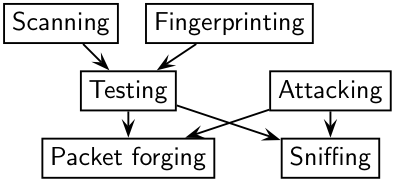
\includegraphics[width=1\linewidth,keepaspectratio]{taxonomy.png}
    \caption{Scapy's taxonomy as depicted in \cite{scapy}}
    \label{fig:taxonomy}
\end{figure}
\FloatBarrier

~
\subsubsection{ARP spoofing}

~\newline
As mentioned in the section \ref{sec:Intro}, the general MITM attack goes 
through 3 main steps: Evesdropping, Positioning and Exploiting. 
\textit{ARP spoofing} played a major role in this project's first and middle 
step.

The ARP protocol is normally used to resolve the specific MAC address associated
with a particular IP, so that packets can reach the intended device - 
translating Layer-3 addresses into Layer-2.
On normal circumstances, the sending device sends an ARP Request to discover the
MAC address of a particular IP.
This request is then broadcasted to the network and the device with the 
specified IP sends an ARP Response announcing its MAC address.

This process can be bypassed by sending an unsolicited ARP Response to a 
specific user, announcing that a particular IP actually belongs to the 
attacker's MAC address.
In the most common form of \textit{ARP spoofing}, the attacker forges an ARP 
Response packet declaring that its MAC address is the one associated with the
active Access Point (AP) IP. 
The attacker then informs the actual AP (in a similar way) that its MAC address
is the one associated with the victims IP.
This way the attacker inserts itself in the middle of all communications 
between the victim and the network, and is able to analyse all the victim's 
traffic.

~
\subsubsection{TCP hijack}

~\newline
An alternative method to accomplish the \textbf{Positioning} step of section
\ref{sec:Intro} is \textit{TCP hijacking}. 

During TCP's three-hand handshake, the client initially sends a random value to
be used as its sequence number (Seq.A), and the server replies with an 
acknowledgment number (ACK) of Seq.A + 1 and a random value value of its own, 
sequence number (Seq.B).
This values are then used to re-arrange out of order packets and ensure that 
the correct packet is received during communication.

An attacker can impersonate one of the involved parties by forging an IP packet 
with the correct ongoing Seq. and ACK values. 
If that happens, the victim's own Seq. and ACK numbers became offsetted, and 
their packets are dropped when reaching the other side of the conversation.
As such, the attacker is able to "hijack" the ongoing connection.

This approach faces some problems: 
\begin{itemize}
    \item \underline{It requires a ongoing connection} - upon receiving a forged
        SYN packet, the server will reply with a SYN ACK to the IP of said 
        packet. 
        Since the real device of this IP did not start a connection, it will
        respond with a TCP packet whose RST bit is set, immediately closing the
        connection.

    \item \underline{The server, and client became aware of the 
        hijack} - it's possible that the large quantity of sudden dropped 
        packets trigger some kind of security alert and this may cause the 
        connection to be dropped.
\end{itemize}

Both these problems can be somewhat dealt with by conditioning not only 
when this attack may occur, but also by closing the real client's connection 
before the hijack, without the server realizing it.

~
\subsubsection{RST attack}

~\newline
Each TCP packet has a header, and each header contains a bit known as the 
"reset" (RST) flag. 
In usual TCP traffic, this bit is set to 0 and has no effect.
However, if this bit is set to 1, it indicates to the receiving device that 
it should immediately stop using the TCP connection; 
it should not send any more packets using the connection's identifying numbers, 
called ports, and discard any further packets it receives with headers 
indicating they belong to this connection. 
A TCP reset basically kills a TCP connection instantly. 

As seen previously, it's possible to inject a forged TCP packet into a ongoing 
TCP connection, if the forged Seq. and ACK numbers are correct. 
As such, an attacker can prematurely terminate a TCP connection, without the 
willing consent of the parties involved.

~
\subsubsection{Reverse Shell}

~\newline
In a typical remote access scenario, the user is the client and the target 
machine is the server. 
The user initiates a remote shell connection and the target system listens 
for such connections. 
With a reverse shell, the roles are the opposite. 
The target machine initiates the connection to the user, and the 
user’s device listens for incoming connections on a specified port.
This can be used to bypass firewall restrictions on open ports, as most 
restrictions are imposed on incoming traffic, not on outgoing one.
Reverse shells can usually be used after some initial code or packet is 
injected in the target machine and allow an attacker to obtain a interactive 
shell session on the victim's machine.
